\documentclass[11pt]{article}

% ---------- Page & fonts ----------
\usepackage[margin=1in]{geometry}
\usepackage[utf8]{inputenc}
\usepackage[T1]{fontenc}

% ---------- Math ----------
\usepackage{amsmath, amssymb, amsthm, mathtools}

% ---------- Graphs / figures ----------
\usepackage{tikz}
\usetikzlibrary{positioning, arrows.meta, calc}

% ---------- Quality of life ----------
\usepackage{enumitem}
\usepackage{hyperref}
\usepackage{cleveref}
\usepackage{xcolor}

\hypersetup{
  colorlinks=true,
  linkcolor=blue!50!black,
  citecolor=blue!50!black,
  urlcolor=blue!50!black
}

% ================= Theorem environments =================
\theoremstyle{plain}
\newtheorem{theorem}{Theorem}[section]
\newtheorem{lemma}[theorem]{Lemma}
\newtheorem{proposition}[theorem]{Proposition}
\newtheorem{corollary}[theorem]{Corollary}
\newtheorem{conjecture}[theorem]{Conjecture}

\theoremstyle{definition}
\newtheorem{definition}[theorem]{Definition}
\newtheorem{example}[theorem]{Example}
\newtheorem{exercise}[theorem]{Exercise}

\theoremstyle{remark}
\newtheorem{remark}[theorem]{Remark}
\newtheorem*{note}{Note}

% ================= Graph theory macros =================
% Sets
\newcommand{\V}{V}                       % vertex set
\newcommand{\E}{E}                       % edge set
\newcommand{\N}{N}                       % neighbourhood, N(v)

% Common graph families
\newcommand{\Kn}[1]{K_{#1}}              % complete graph K_n
\newcommand{\Kmn}[2]{K_{#1,#2}}          % complete bipartite K_{m,n}
\newcommand{\Cn}[1]{C_{#1}}              % cycle
\newcommand{\Pn}[1]{P_{#1}}              % path

% Invariants (as operators, upright text, correct spacing)
\DeclareMathOperator{\dg}{d}             % degree, use dg(v) to avoid clashing with \deg
\DeclareMathOperator{\ex}{ex}            % extremal function ex(n, H)
\DeclareMathOperator{\girth}{girth}
\DeclareMathOperator{\diam}{diam}
\DeclareMathOperator{\Aut}{Aut}
\DeclareMathOperator{\chr}{\chi}          % chromatic number, use \chr(G)
\DeclareMathOperator{\comp}{c}            % number of components

% Misc shorthands
\newcommand{\iso}{\cong}                 % isomorphic
\newcommand{\subgraph}{\subseteq}        % spanning/sub relations, adjust as needed

% ================= Document =================
\title{Graph Theory Notes}
\author{}
\date{\today}

\begin{document}

\maketitle

\section{Topic}

% ---------- Definition block ----------
\begin{definition}[Name]
  Statement of the definition.
\end{definition}

% ---------- Example with a tikz figure ----------
\begin{example}
  A small example graph.
  \begin{center}
    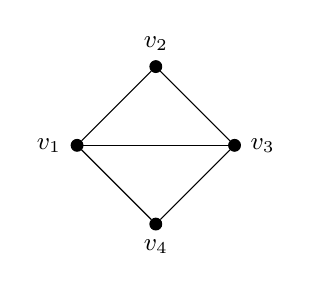
\begin{tikzpicture}[
        vertex/.style={circle, draw, fill=black, inner sep=1.5pt},
        every node/.style={font=\small}
      ]
      \node[vertex, label=left:$v_1$]  (v1) at (0, 0)   {};
      \node[vertex, label=above:$v_2$] (v2) at (1, 1)   {};
      \node[vertex, label=right:$v_3$] (v3) at (2, 0)   {};
      \node[vertex, label=below:$v_4$] (v4) at (1, -1)  {};

      \draw (v1) -- (v2);
      \draw (v2) -- (v3);
      \draw (v3) -- (v4);
      \draw (v4) -- (v1);
      \draw (v1) -- (v3);
    \end{tikzpicture}
  \end{center}
\end{example}

% ---------- Theorem / proof block ----------
\begin{theorem}[Name or attribution]
  Statement of the theorem.
\end{theorem}

\begin{proof}
  Proof goes here. \qedhere
\end{proof}

% ---------- Remark ----------
\begin{remark}
  Optional side comment, intuition, or a pointer to a related result.
\end{remark}

\end{document}